\chapter{Related Work}

This chapter highlights the theories and recent advancements in the fields of remote sensing and computer vision, particularly in small object detection.
By examining previous research that addresses those challenges, this section not only underscores the technological progress achieved but also identifies 
the gaps that the current model aims to bridge. In the field of computer vision, Convolutional Neural Networks (CNNs) served as the initial models for 
image analysis, primarily focused on image classification where the entire image is labeled as a single object category. While CNNs had great performance 
in these tasks, their application to object detection in complex images revealed significant limitations.

Object detection models can be broadly categorized by annotation method into anchor-based and anchor-free approaches, and by detection method into dense 
prediction (single-stage) and sparse prediction (multi-stage) techniques. This categorization helps in understanding the diverse strategies employed in 
detecting objects across different scenarios.

This chapter begins with the foundational R-CNN model, which introduced the use of convolutional networks for robust object detection. The following sections 
dive into Fast R-CNN and Faster R-CNN, which iteratively refined the integration of region proposal mechanisms with deep learning, significantly enhancing 
detection efficiency and speed. The exploration continues with Mask R-CNN and Feature Pyramid Networks, which extended capabilities to instance segmentation 
and improved feature representation at multiple scales, respectively.

Single-stage detection models, or dense prediction models, such as YOLO (You Only Look Once) and SSD (Single Shot MultiBox Detector), streamline the detection 
process by eliminating the need for a separate region proposal step. These models directly predict object classes and bounding box coordinates from full 
images in one evaluation, optimizing for speed and efficiency.

The latter sections of the chapter explore cutting-edge developments like the Vision Transformer and Masked-Attention Mask Transformer, which incorporate 
transformer architectures to push the boundaries of object detection and segmentation.



\section{Multi-stage Object Detection Models}

Multi-stage object detection models involve a more complex process that typically includes distinct phases for generating region proposals and then classifying 
these proposals into specific object categories. These models first isolate potential object locations before applying sophisticated classification and 
bounding box regression techniques. This separation allows for more precise detections and higher overall accuracy, making multi-stage models adept at 
handling complex image scenarios with multiple objects and varying scales. The trade-off, however, is usually slower processing speeds compared to 
single-stage detectors.

\subsection{Region-based Convolution Neural Networks}

The R-CNN family of models represents a fundamental shift in object detection, introducing deep learning to generate high-quality region proposals 
that are then classified by a convolutional neural network. This evolutionary path not only streamlined the detection pipeline but also improved the 
scalability and applicability of these models in real-world scenarios, where speed and accuracy are crucial. The successive refinements from R-CNN 
through Mask R-CNN highlight a trajectory of continuous improvement, with  each iteration bringing more sophisticated integration of features and functionalities.


\newpage
\subsubsection{Region-based Convolution Neural Networks}

The need for more sophisticated solutions that could accurately identify and locate multiple objects within images led to the development of 
Region-based Convolutional Networks[3] (R-CNNs). Starting with the base Region-based Convolution Neural Network This approach combines region proposal 
algorithms with the feature extraction capabilities of CNNs. R-CNNs begin by generating potential object-bound regions in an image, a process known 
as region proposal. Each region is then cropped and resized to a fixed size before being fed into a pre-trained convolutional neural network. 

\begin{figure}[h!]
    \centering
    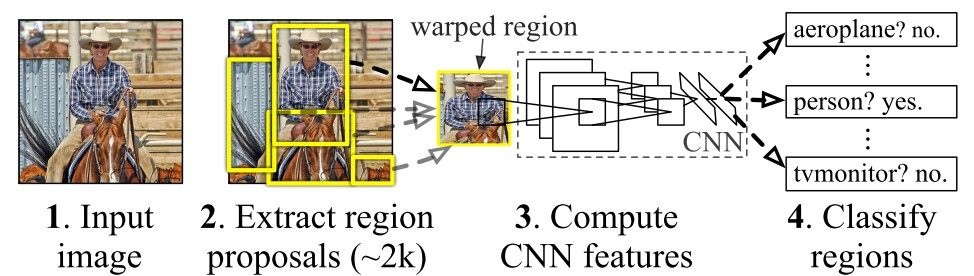
\includegraphics[scale=0.45]{Figures/rcnn.jpeg}
    \caption{Region-based Convolution Neural Network Architecture}
    \label{fig:rcnn}
\end{figure}

As presented in the \ref{fig:rcnn} the R-CNN consists of 3 main modules. The first module generates 2,000 region proposals using the Selective Search 
algorithm. After being resized to a fixed pre-defined size, the second module extracts a feature vector of length 4,096 from each region proposal.
The third module uses a pre-trained SVM algorithm to classify the region proposal to either the background or one of the object classes.


Some the limitations of the R-CNN model are the facts that it is a multi-stage model, where each stage is an independent component, thus, it cannot be 
trained end-to-end. Also the R-CNN depends on the Selective Search algorithm for generating region proposals, which takes a lot of time and cannot be 
customized to the detection problem. Lastly each region proposal is fed independently to the CNN for feature extraction, which makes it impossible to 
run R-CNN in real-time.

\subsubsection{Fast Region-based Convolution Neural Networks}

Fast R-CNN improved upon the original R-CNN's efficiency, where instead of cropping and resizing each region separately, the entire image is passed through the 
CNN to extract features. Regions of interest (ROIs) are then selected from the feature map using the proposed bounding boxes from the selective search. 
These ROIs are then pooled into a fixed-size feature map and passed through fully connected layers for classification and bounding box regression 
in the figure \ref{fig:fast-rcnn}.

\begin{figure}[h!]
    \centering
    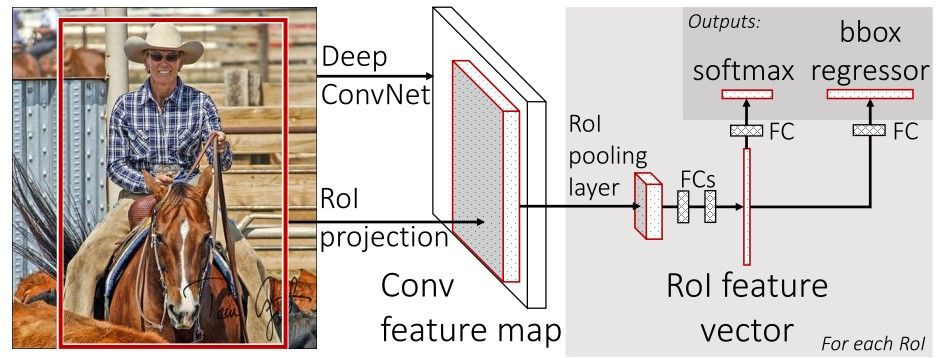
\includegraphics[scale=0.4]{Figures/fast-r-cnn.png}
    \caption{Fast Region-based Convolution Neural Network Architecture}
    \label{fig:fast-rcnn}
\end{figure}

In this model a proposed a new layer called ROI Pooling that extracts equal-length feature vectors from all proposals in the same image, where 
compared to R-CNN, which has multiple stages, Faster R-CNN builds a network that has only a single stage. 

\newpage
The RoI pooling layer uses max pooling to convert the features inside any valid region of interest into a small feature map with a fixed spatial 
extent of \(H \times W\) , where $H$ and $W$ are layer hyper-parameters that are independent of any particular RoI. In this paper, an RoI is a rectangular window 
into a convolution feature map. Each RoI is defined by a four-tuple \((r, c, h, w)\) that specifies its top-left corner \((r, c)\) and its height 
and width \((h, w)\). Also one of the great inclusions of this model was the implementation of multi-task loss:

\[L(p, u, t', v) = L_{cls}(p, u) + \lambda [u \geq 1] L_{loc}(t', v)z\]

,where the classification loss \(L_{cls}(p, u)\) is defined as the negative log likelihood of the true class \(u\), expressed as:
\[
L_{cls}(p, u) = -\log p_u
\]

The localization loss \(L_{loc}\) is defined over the predicted bounding box parameters \(t' = (t'_x, t'_y, t'_w, t'_h)\) and the ground truth bounding 
box parameters \(v = (v_x, v_y, v_w, v_h)\) for class \(u\). The Iverson bracket \([u \geq 1]\) is used as an indicator function that evaluates to 1 
when \(u\) is 1 or more, and 0 otherwise. This function helps in applying the localization loss only when there is a foreground class detected, 
effectively ignoring the background.

The overall loss \(L(p, u, t', v)\) is then a combination of classification and localization losses, modulated by a parameter \(\lambda\), representing the trade-off between these two tasks:
\[
L(p, u, t', v) = L_{cls}(p, u) + \lambda [u \geq 1] L_{loc}(t', v)
\]

\newpage
\subsubsection{Faster Region-based Convolution Neural Networks}

While Fast R-CNN improved upon its predecessors in terms of both speed and accuracy, the Faster R-CNN[4] architecture emerged as an even more refined version. 
Fast R-CNN effectively addressed the inefficiencies of previous models by integrating a region of interest (RoI) pooling layer to connect convolutional 
feature extraction and region proposal tasks. However, it still relied on external region proposal algorithms, which remained a bottleneck in terms of 
computational efficiency and speed. 

\begin{figure}[h!]
    \centering
    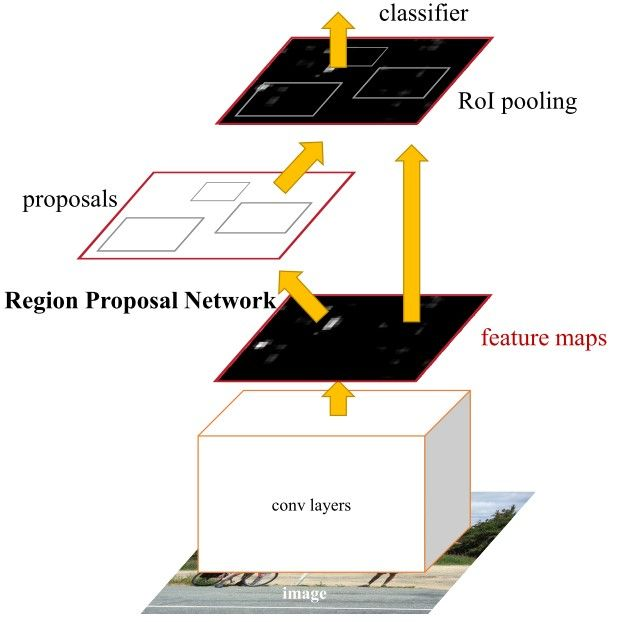
\includegraphics[scale=0.4]{Figures/faster-rcnn.jpeg}
    \caption{Faster Region-based Convolution Neural Network Architecture}
    \label{fig:faster-rcnn}
\end{figure}

Faster R-CNN resolved this by introducing a novel component, the Region Proposal Network (RPN)[5]. A Region Proposal Network takes an image
(of any size) as input and outputs a set of rectangular object proposals, each with an objectness score. This process is modeled with a fully 
convolutional network, because the ultimate goal is to share its computation with a Fast R-CNN object detection network, as it is assumed that 
both nets share a common set of convolutional layers, as seen in the Figure \ref{fig:faster-rcnn}.


To generate region proposals, a small network slides over the convolutional feature map output by the last shared convolutional layer. This small
network takes as input an $n \times n$ spatial window of the input convolutional feature map. Each sliding window is mapped to a lower-dimensional feature.
This feature is fed into two sibling fully-connected layers—a box-regression layer (reg layer) and a box-classification layer (cls layer). This mini-network 
is illustrated at a single position in the Figure \ref{fig:anchors}. Also since the mini-network operates in a sliding-window fashion, the 
fully-connected layers are shared across all spatial locations. 

This architecture is naturally implemented with an n×n convolutional layer followed by two sibling $1 \times 1$ convolutional layers. 

\newpage
At each sliding-window 
location, there is simultaneously a prediction of multiple region proposals, where the number of maximum possible proposals for each location is
denoted as k. The k proposals are parameterized relative to k reference boxes, which are called  anchors. An anchor is centered at the sliding window
in question, and is associated with a scale and aspect ratio as seen again in Figure \ref{fig:anchors}. By default 3 scales and 3 aspect ratios are used, 
yielding k = 9 anchors at each sliding position. For a convolutional feature map of a size $W \times H$, there are $W \times H \times k$ anchors in total.

\begin{figure}
    \centering
    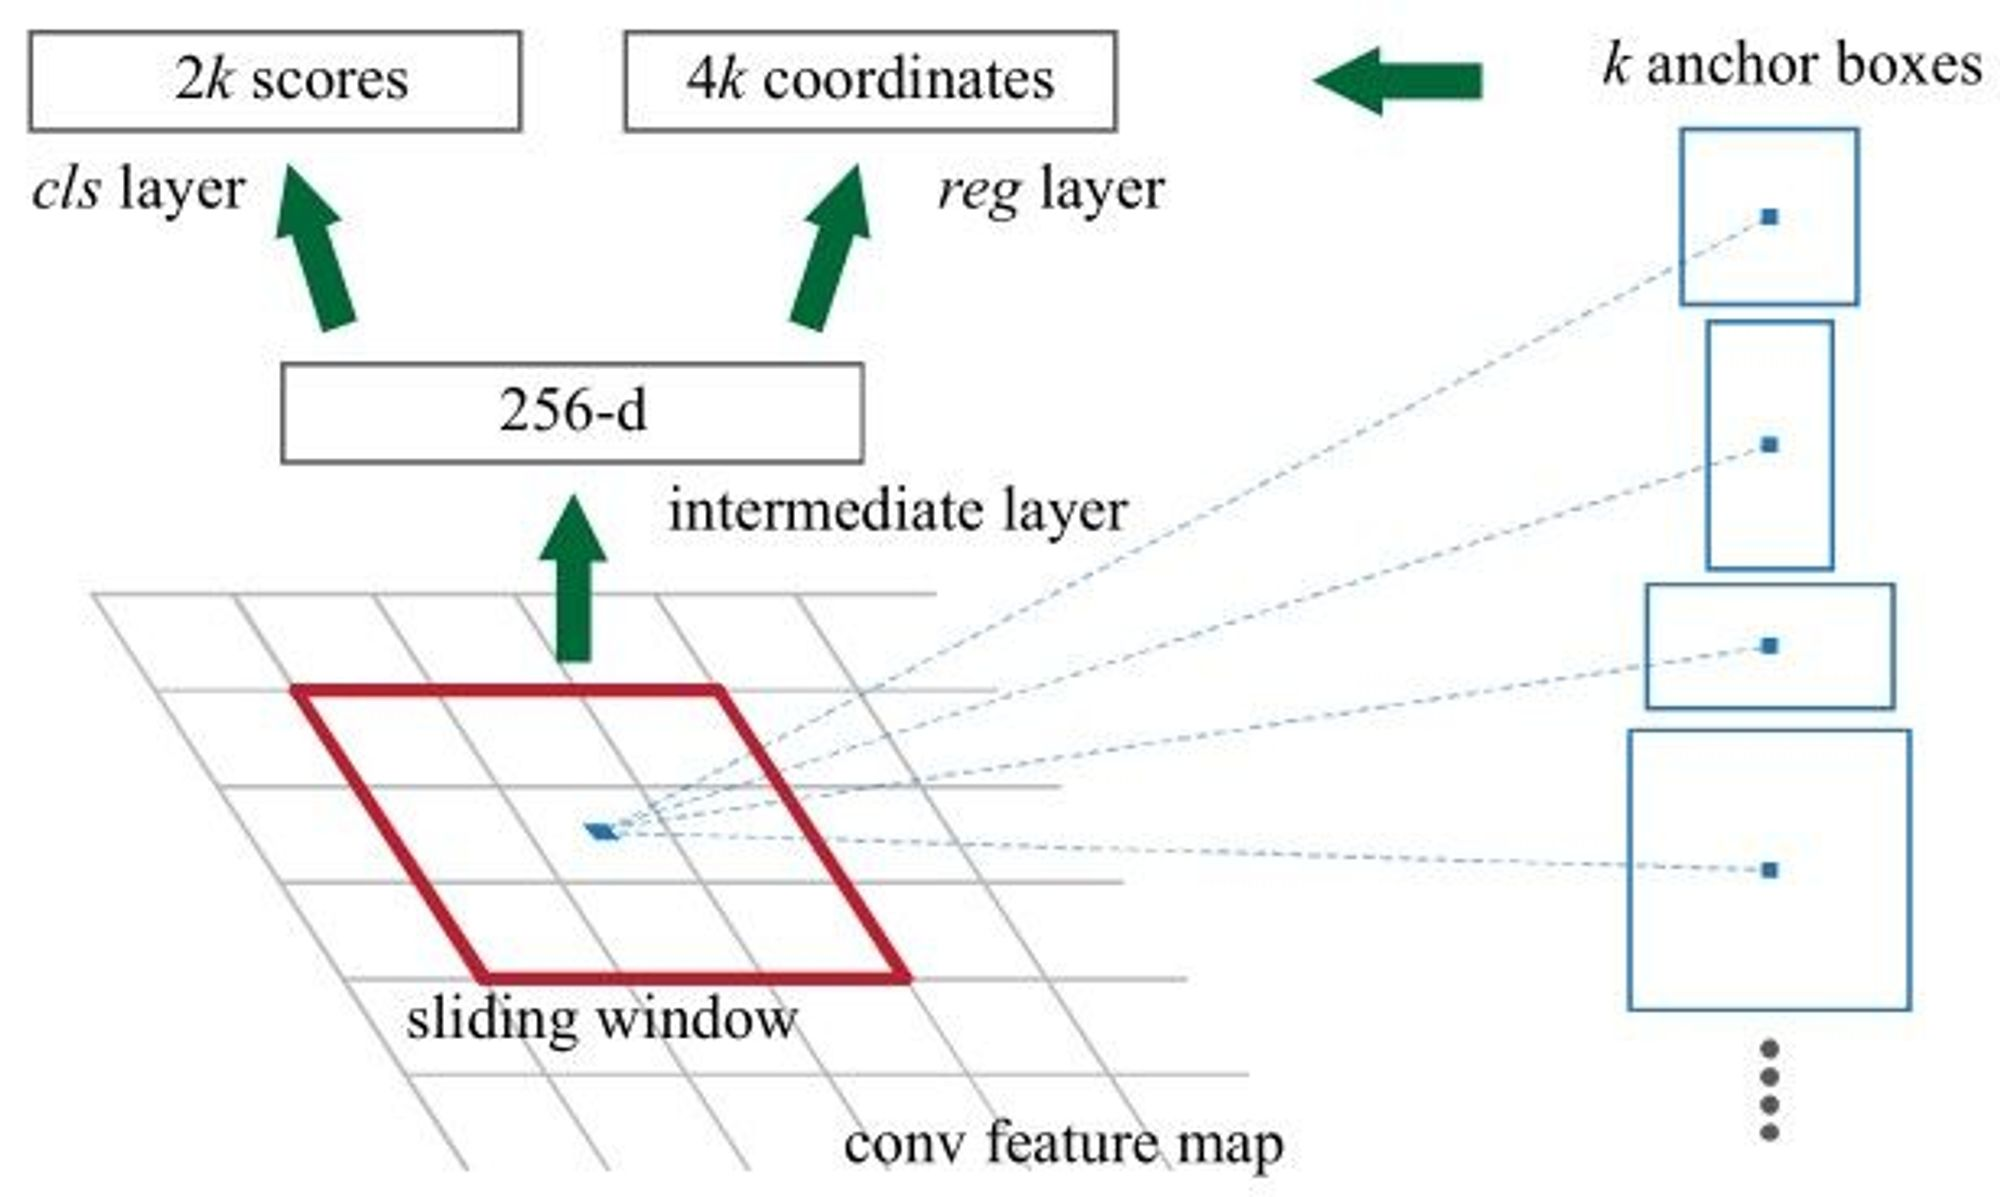
\includegraphics[scale=0.1]{Figures/anchors.jpeg}
    \caption{Region Proposal Network}
    \label{fig:anchors}
\end{figure}


\subsubsection{Masked Region-based Convolution Neural Networks}

Mask R-CNN builds on the ideas and successes of the Faster R-CNN model, which predicts both a class label and a bounding-box offset for each candidate object. 
To these, Mask R-CNN adds a third branch specifically designed to output the object mask, providing a straightforward and logical extension to the 
existing framework. This addition allows Mask R-CNN to capture the precise spatial layout of objects, a task that necessitates extracting significantly 
finer detail than what is required for classifying objects or predicting bounding boxes alone.

Mask R-CNN adopts the same two-stage procedure as Faster R-CNN, with an identical first stage the RPN. In the second stage, in parallel to predicting 
the class and box offset, Mask R-CNN also outputs a binary mask for each RoI. This is in contrast to most recent systems, where classification 
depends on mask predictions. This approach follows the spirit of Fast R-CNN that applies bounding-box classification and regression in parallel.


\begin{figure}[h!]
    \centering
    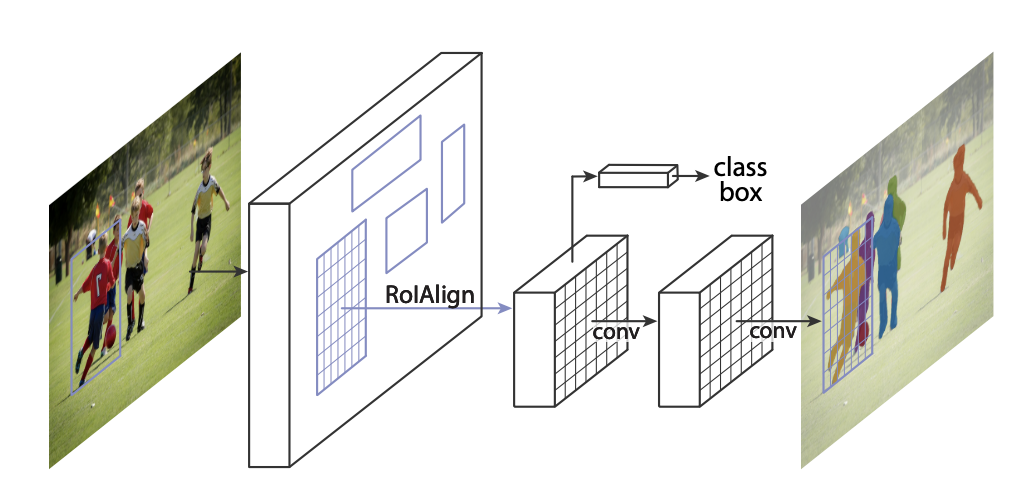
\includegraphics[scale=0.5]{Figures/mask-r-cnn.png}
    \caption{Mask Region Convolution Neural Network Architecture}
    \label{fig:mask-r-cnn}
\end{figure}

\newpage
A mask encodes an input object’s spatial layout. Thus, unlike class labels or box offsets that are inevitably collapsed into short output vectors by
fully-connected layers, extracting the spatial structure of masks can be addressed naturally by the pixel-to-pixel correspondence provided by convolutions.
Specifically, an $m \times m$ mask is predicted from each RoI using an FCN. This allows each layer in the mask branch to maintain the explicit $m \times m$ object 
spatial layout without collapsing it into a vector representation that lacks spatial dimensions. Unlike previous methods that resort to fully-connected layers 
for mask prediction, this fully convolutional representation requires fewer parameters, and is more accurate as demonstrated by experiments.

This pixel-to-pixel behavior requires our RoI features, which themselves are small feature maps, to be well aligned to faithfully preserve the explicit 
per-pixel spatial correspondence. This motivated us to develop the following RoIAlign layer that plays a key role in mask prediction.

RoIPool is a standard operation for extracting a small feature map like \(7 \times 7\) from each RoI. RoIPool first quantizes a floating-number RoI to the 
discrete granularity of the feature map, this quantized RoI is then subdivided into spatial bins  which are themselves quantized, and finally feature 
values covered by each bin are aggregated usually by max pooling. 

Quantization, such as that performed on a continuous coordinate $x$ by calculating \(\frac{x}{16}\), where 16 represents the feature map stride accompanied
by the rounding. Similarly, this quantization process occurs when coordinates are divided into discrete bins, for example, into a $7x7$ grid. However, these 
quantization steps can lead to slight misalignments between the Region of Interest (RoI) and the features extracted from it, potentially affecting the accuracy 
of the model.

\begin{figure}[h!]
    \centering
    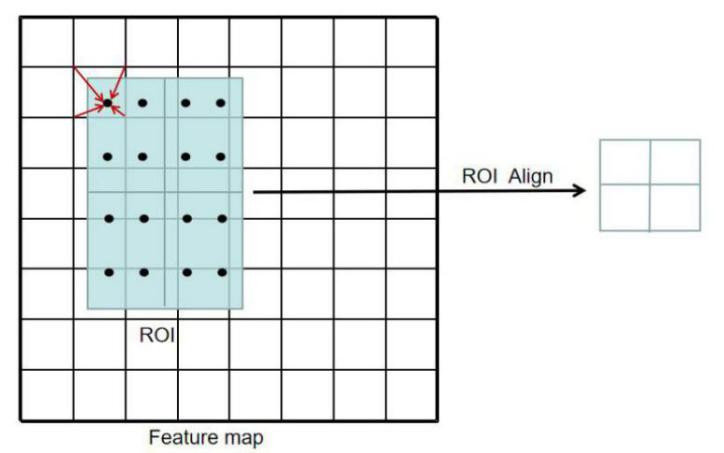
\includegraphics[scale=0.35]{Figures/mask-r-cnn-roi-align.png}
    \caption{Mask Region Of Interest}
    \label{fig:roi-align}
\end{figure}

While this may not impact classification, which is robust to small translations, it has a large negative effect on predicting pixel-accurate masks.
To address this, a RoIAlign layer is proposed that removes the harsh quantization of RoIPool, properly aligning the extracted features with the input. 
A bilinear interpolation is used to compute the exact values of the input features at four regularly sampled locations in each RoI bin, and aggregate 
the result.

\newpage
Furthermore once again this model utilizes a multi-task loss in order to take into consideration all the outputs of the model.
\[
L = L_{cls} + L_{box} + L_{mask} 
\]
 
The mask branch has a $K \times m^2$-dimensional output for each RoI, which encodes K binary masks of resolution m × m, one for each of the K classes.
To this a per-pixel sigmoid is applied, and define Lmask as the average binary cross-entropy loss. For an RoI associated with ground-truth class k, 
$L_{mask}$ is only defined on the k-th mask. This definition of $L_{mask}$ allows the network to generate masks for every class without competition 
among classes, since on the dedicated classification branch to predict the class label used to select the output mask. This decouples mask and 
class prediction. This is different from common practice when applying FCNs to semantic segmentation, which typically uses a per-pixel softmax and a 
multinomial cross-entropy loss. In that case, masks across classes compete; in our case, with a per-pixel sigmoid and a binary
loss, they do not.


\subsection{Feature Pyramid Networks}

The concept of Feature Pyramid Networks (FPNs) was a significant advancement in object detection and segmentation, by leveraging the inherent multi-scale, 
pyramidal hierarchy of deep convolutional networks. The first subsection details the basic Feature Pyramid Network, an architecture that efficiently creates 
a pyramid of features at multiple levels, enabling the detection of objects at various scales with improved accuracy. This structure uses a top-down approach 
with lateral connections to combine low-resolution, semantically strong features with high-resolution, semantically weaker features, enhancing the network’s 
ability to detect objects across different scales. The subsequent subsection explores the Extended Feature Pyramid Network, which builds upon the original FPN 
by introducing enhancements that further refine feature integration and improve detection performance, particularly in challenging scenarios with complex object 
orientations and scales.


\subsubsection{Feature Pyramid Network}

With Feature Pyramid Networks the objective is to harness the pyramidal feature hierarchy of a Convolutional Networks, which inherently contains semantic 
information from low to high levels, to construct a feature pyramid that maintains high-level semantics throughout. The method processes a single-scale 
image of arbitrary size and produces proportionally sized feature maps at multiple levels, utilizing a fully convolutional approach. This procedure is 
compatible with various backbone convolutional architectures, and this paper demonstrates results using ResNets. The construction of the pyramid incorporates 
a bottom-up pathway, a top-down pathway, and lateral connections, which are detailed below and seen in the Figure \ref{fig:fpn}.

The bottom-up pathway is the feed forward computation of the ConvNet backbone, which computes a feature hierarchy consisting of feature maps at several scales 
with a scaling step of 2. There are often many layers producing output maps of the same size and these layers are in the same network stage. For the 
feature pyramid, one pyramid level for each stage is defined. The output of the last layer of each stage is chosen as the reference set of feature maps, 
which will be enriched to create the pyramid. This choice is logical because the deepest layer of each stage is expected to have the strongest features.

Specifically, for ResNets, the feature activations output by the last residual block of each stage are utilized. These outputs are denoted as ${C2, C3, C4, C5}$ 
corresponding to the outputs of conv2, conv3, conv4, and conv5, respectively. It is important to note that these have strides of ${4, 8, 16, 32}$ pixels with 
respect to the input image. The conv1 output is not included in the pyramid due to its large memory footprint.

\begin{figure}[h!]
    \centering
    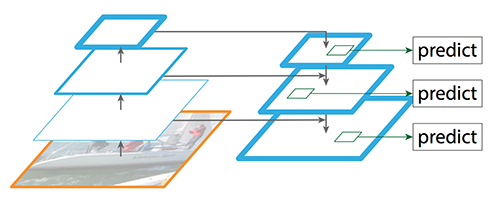
\includegraphics[scale=0.35]{Figures/fpn-base.png}
    \caption{Feature Pyramid Network}
    \label{fig:fpn}
\end{figure}

The top-down pathway hallucinates higher resolution features by up-sampling spatially coarser, but semantically stronger, feature maps from higher pyramid levels. 
These features are then enhanced with features from the bottom-up pathway via lateral connections. Each lateral connection merges feature maps of the same 
spatial size from the bottom-up pathway and the top-down pathway. The bottom-up feature map is of lower-level semantics, but its activations are more accurately 
localized as it was sub-sampled fewer times. With a coarser-resolution feature map, the spatial resolution is up-sampled by a factor of 2. The up-sampled map is 
then merged with the corresponding bottom-up map (which undergoes a 1×1 convolutional layer to reduce channel dimensions) by element-wise addition 
as seen in the figure \ref{fig:fpn-top}. This process is iterated until the finest resolution map is generated. To start the iteration, simply attach a 
1×1 convolutional layer on $C5$ to  produce the coarsest resolution map. 

\begin{figure}[h!]
    \centering
    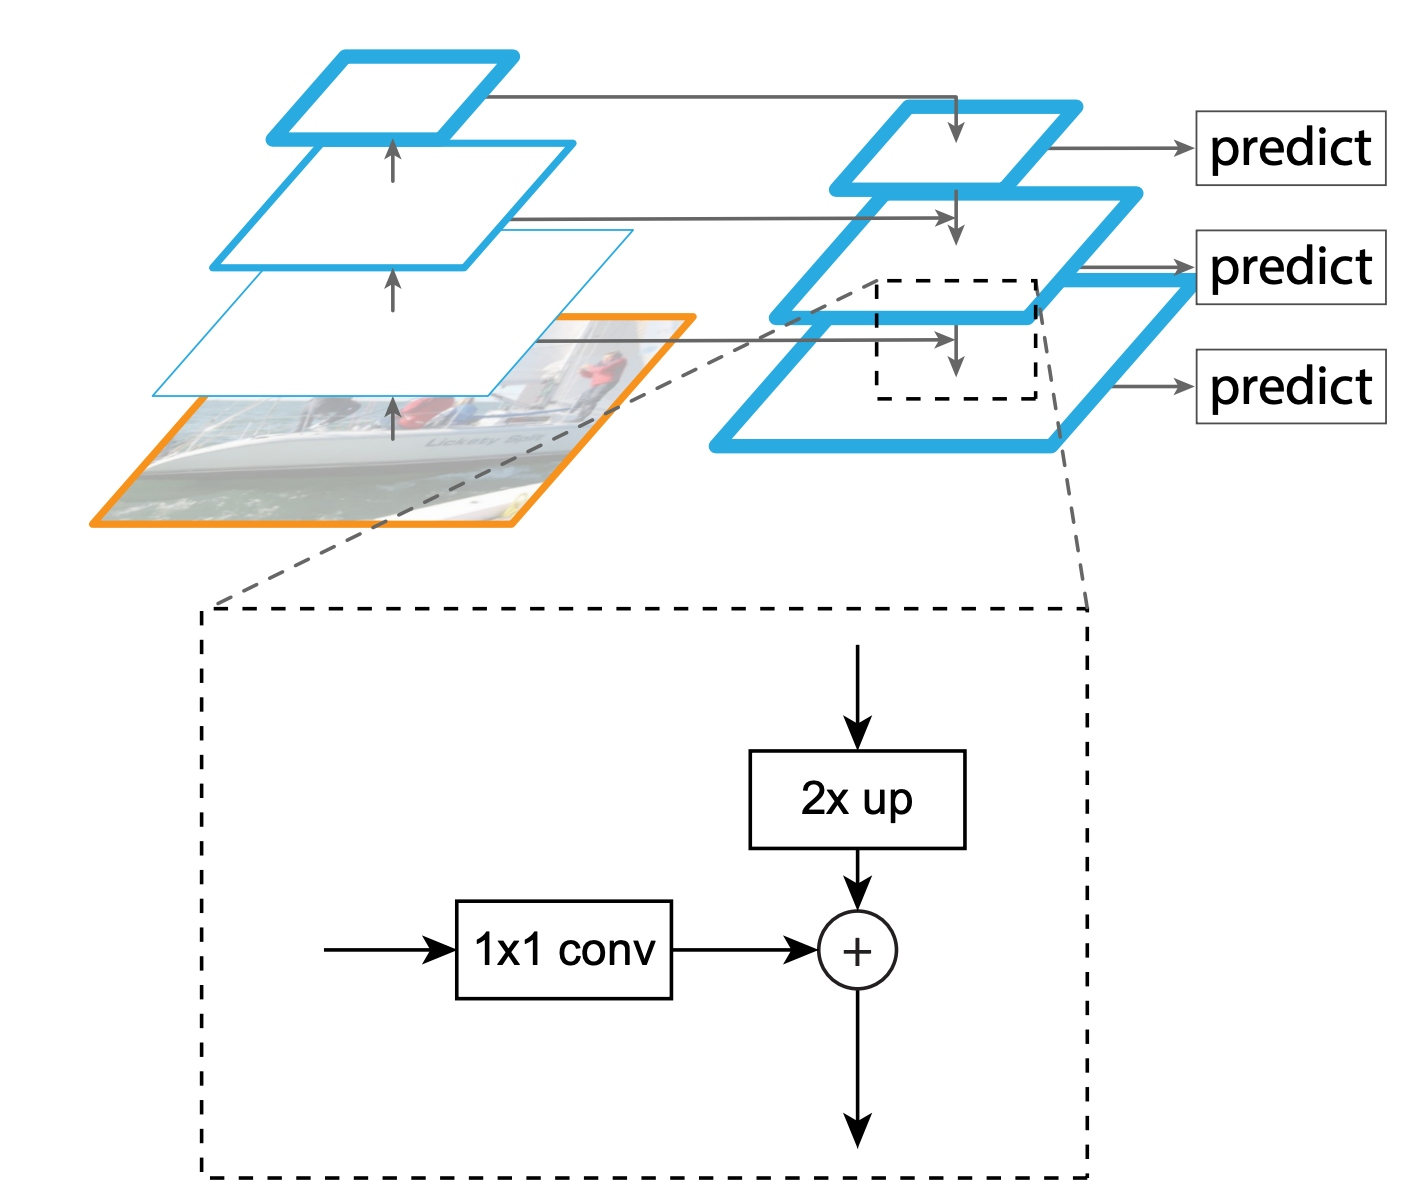
\includegraphics[scale=0.35]{Figures/fpn-top-down.jpg}
    \caption{}
    \label{fig:fpn-top}
\end{figure}


Finally a 3×3 convolution is added on each merged map to generate the final feature map, which is to reduce the aliasing effect of up-sampling. 
This final set of feature maps is called ${P2, P3, P4, P5}$, corresponding to ${C2, C3, C4, C5}$ that are respectively of the same spatial sizes.
Since all levels of the pyramid use shared classifiers/regressors as in a traditional featurized image pyramid, a fixed feature dimension 
or numbers of channels is set, with the value being denoted as $d$ in all the feature maps. With $d = 256$ in this paper and thus all extra convolutional 
layers have 256-channel outputs. Simplicity is central to this design and it has been proven that this model is robust to many design choices. We have 
experimented with more sophisticated  blocks and observed marginally better results. Designing better connection modules is not the focus of this paper, 
so we opt for the simple design described above.


\subsection{Vision Transformers}









\section{Single-stage Object Detection Models}

Single-stage object detection models represent a streamlined approach to identifying and localizing objects within an image. Unlike multi-stage models, 
single-stage models, such as YOLO (You Only Look Once) and SSD (Single Shot MultiBox Detector), operate in a direct manner by predicting object classes and 
bounding box coordinates in a single forward pass through the network. This methodology not only simplifies the detection pipeline but also enhances the 
speed of detection, making single-stage models particularly well-suited for real-time applications. However, this increase in speed can sometimes come at 
the cost of lower accuracy, especially in detecting small or overlapping objects.

\subsection{You Only Look Once}

\subsection{Single Shot MultiBox Detector}

